\section{Free Software: a Prison Break}

\begin{frame}
  \frametitle{Free Software: a Prison Break}

  \begin{itemize}
    \item Free Software: Four Essential Freedoms
    \item A bit about History
    \item GNU/Linux
  \end{itemize}
  
  \centering
  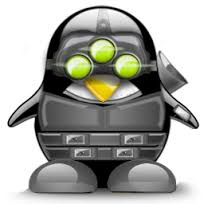
\includegraphics[width=2.5cm]{tux_sc}
  
\end{frame}




\begin{frame}
  \frametitle{Free Software: Four Essential Freedoms}

  \begin{itemize}
    \item
         A program is considered free when its license offers to all its
users the following four freedoms
\begin{itemize}
    \item 
Freedom to \textbf{run} the software for \textbf{any purpose}
\item Freedom to \textbf{study} the software and to \textbf{change} it
\item Freedom to \textbf{redistribute} copies
\item Freedom to \textbf{distribute} copies of \textbf{modified versions}
\end{itemize}
\item These freedoms are granted for both commercial and
non-commercial use
\item They imply the availability of source code, software can be
modified and distributed to customers
\item \textbf{Good match for embedded systems!}
  \end{itemize}
  
\end{frame}



\begin{frame}
  \frametitle{A bit about History}
  
    \begin{itemize}
        \item \textbf{1983}, Richard Stallman, \textbf{GNU} project and the free software
concept. Beginning of the development of gcc, gdb, glibc and
other important tools
\item \textbf{1991}, Linus Torvalds, \textbf{Linux kernel} project, a Unix-like
operating system kernel. Together with GNU software and
many other open-source components: a completely free
operating system, \textbf{GNU/Linux}
\item \textbf{1995}, Linux is more and more popular on server systems
\item \textbf{2000}, Linux is more and more popular on embedded
systems
\item \textbf{2008}, Linux is more and more popular on mobile devices
\item \textbf{2010}, Linux is more and more popular on phones
    \end{itemize}
  
  
\end{frame}



\begin{frame}
  \frametitle{GNU/Linux}
  
  \begin{block}{Richard Stallman}
   What you guys are referring to as Linux, is in fact, GNU/Linux, or as I've recently taken to calling it, GNU plus Linux. Linux is not an operating system unto itself, but rather another free component of a fully functioning GNU system made useful by the GNU corelibs, shell utilities and vital system components comprising a full OS as defined by POSIX.
  \end{block}
  
    \centering
  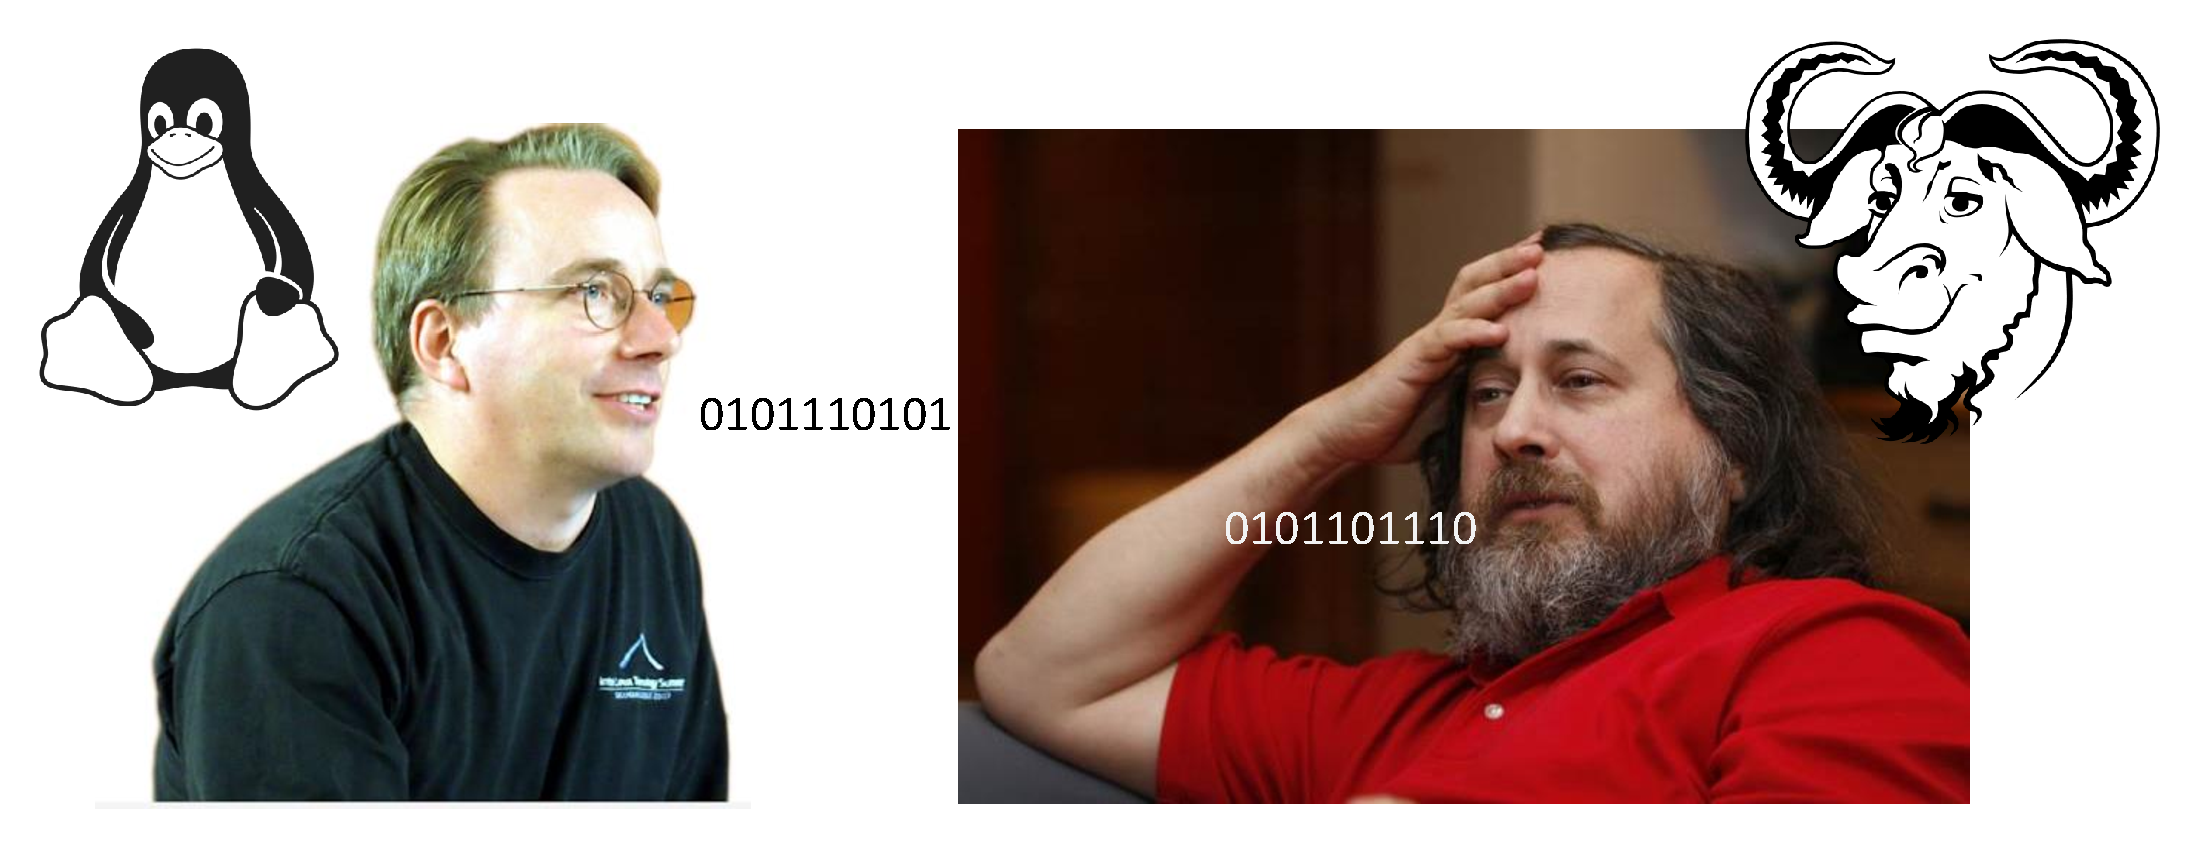
\includegraphics[width=8cm]{controversy}
  
\end{frame}

